\section{Architecture}
In this section it is described the architecture of the plant monitoring system application. All the following steps has been made by using the guide developed by Laurent Deru, Sébastien Dawans and Mathieu Ocana, available in GitHub under permissive 3-clause BSD-style open source license. However, in the tutorial it is used only TelosB node instead of the Texas Instrument Sensor Tags. Using the TI nodes is the overall greatest challenge described in this paper.\\
\subsection{The network}
The network main idea is well depicted in figure \ref{fig:Network}. The raspberry pi act as a six low pan border router (6LBR) and act as a link between the Ethernet and the wireless sensor network. The wireless sensor network is composed by the TelosB that act as a sink for all the other sensor tags. The TelosB sensor is attached via USB to the Raspberry Pi.
\begin{figure}[!h]
	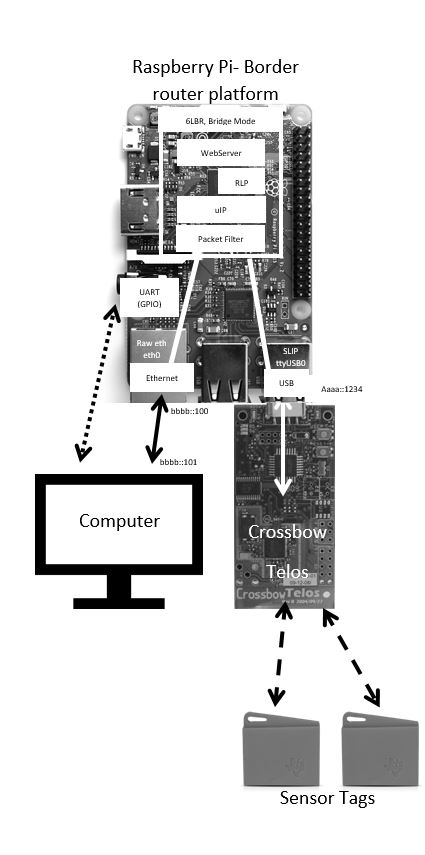
\includegraphics[width=\linewidth]{Network}
	\caption{Development of the network}
	\label{fig:Network}
\end{figure}
On the other hand, the Raspberry Pi is connected to a computer via a normal house router.\cite{6lbr}
The Raspberry Pi connect the two subnets via RPL protocol on the wireless sensor network side and NPD on the Ethernet part.\cite{mode}\\

\subsection{CoAP}
Before commence the description of web server, it is very essential an explanation of CoAP. CoAP stands for Constarined Application Protocol. It is an application protocol used for transfer information as it is HTTP. It works as client/server model where a server send after the client request. However, it differ from HTTP because of the constrained resource devices where CoAP works. CoAP is designed for limit the consume of RAM, the packet are much smaller. \cite{coap}

\subsection{WebServer}




